\documentclass[11pt]{article}
% ===========================================================================
%  Shared preamble for all MPM2D worksheets — input right after \documentclass.
%  (Files beginning with "_" are skipped by mpm2d-worksheet-publish.mjs.)
% ===========================================================================
\usepackage[letterpaper,top=2.2cm,bottom=1.9cm,left=1.6cm,right=1.6cm,headheight=28pt,footskip=24pt]{geometry}
\usepackage{amsmath,amssymb}
\usepackage{cancel}
\usepackage[T1]{fontenc}
\usepackage[utf8]{inputenc}
\usepackage{lmodern}
\usepackage{xcolor}
\usepackage[most]{tcolorbox}
\usepackage{enumitem}
\usepackage{multicol}
\usepackage{fancyhdr}
\usepackage{tikz}
\usetikzlibrary{calc}
\usepackage{pgfplots}
\pgfplotsset{compat=1.18}

\definecolor{exblue}{HTML}{4A90E2}
\definecolor{exbg}{HTML}{E6F3FF}
\definecolor{qorange}{HTML}{E69138}
\definecolor{qbg}{HTML}{FFF7CC}
\definecolor{keygray}{HTML}{475569}
\definecolor{keybg}{HTML}{F1F5F9}
\definecolor{iagreen}{HTML}{14653B}
\definecolor{titleblue}{HTML}{1D4ED8}
% Rotating palette so each worked example gets its own colour.
\definecolor{ex0}{HTML}{2563A0}\definecolor{ex1}{HTML}{3B7D3B}\definecolor{ex2}{HTML}{8A5A00}
\definecolor{ex3}{HTML}{A3327A}\definecolor{ex4}{HTML}{6D28A3}\definecolor{ex5}{HTML}{B08900}
\definecolor{ex6}{HTML}{0E7490}\definecolor{ex7}{HTML}{9A3412}\definecolor{ex8}{HTML}{15803D}

\pagestyle{fancy}
\fancyhf{}
\fancyhead[L]{\footnotesize NAME: \underline{\hspace{3.4cm}}}
\fancyhead[C]{\textbf{Integration Academy}\\[-2pt]{\scriptsize Math Simplified \textperiodcentered{} Success Amplified}}
\fancyhead[R]{\footnotesize MPM2D}
\fancyfoot[L]{\scriptsize dr.merie@IntegrationAcademy.ca}
\fancyfoot[C]{\scriptsize\thepage}
\fancyfoot[R]{\scriptsize IntegrationAcademy.ca}
\renewcommand{\headrulewidth}{1.2pt}
\renewcommand{\footrulewidth}{0.4pt}
\setlength{\parindent}{0pt}
\setlength{\parskip}{4pt}

% Examples are NOT breakable, so each example + its solution stays on one page.
\newtcolorbox{example}[2]{colframe=#1,colback=#1!7,coltitle=white,colbacktitle=#1,fonttitle=\bfseries,title={#2},arc=3pt,boxrule=1pt}
\newtcolorbox{qbox}[1]{colframe=qorange,colback=qbg,coltitle=white,colbacktitle=qorange,fonttitle=\bfseries,title={#1},arc=3pt,breakable,boxrule=1pt}
\newtcolorbox{keybox}{colframe=keygray,colback=keybg,coltitle=white,colbacktitle=keygray,fonttitle=\bfseries,title={$\checkmark$\ Answer Key},arc=3pt,breakable,boxrule=1pt}
\newtcolorbox{recapbox}{colframe=keygray,colback=keybg,coltitle=white,colbacktitle=keygray,fonttitle=\bfseries,title={Question Recap},arc=3pt,breakable,boxrule=1pt}
\newtcolorbox{ideabox}{colframe=titleblue,colback=titleblue!6,coltitle=white,colbacktitle=titleblue,fonttitle=\bfseries,title={The Big Ideas},arc=3pt,breakable,boxrule=1.2pt}
\newtcolorbox{learnbox}{colframe=iagreen,colback=iagreen!5,coltitle=white,colbacktitle=iagreen,fonttitle=\bfseries,title={The Big Picture},arc=3pt,breakable,boxrule=1.2pt}
\newcommand{\lh}[1]{\par\smallskip{\bfseries\color{iagreen}#1}\par\nobreak\smallskip}

\newcommand{\soln}{\par\smallskip\textit{\textbf{Solution.}}\ }
\newcommand{\workspace}[1]{\par\vspace{3pt}\fcolorbox{black!30}{white}{\begin{minipage}[t][#1][t]{\dimexpr\linewidth-2\fboxsep\relax}\ \end{minipage}}\par}
\newcommand{\sech}[1]{\par\vspace{8pt}{\Large\bfseries\color{iagreen}#1}\par\nobreak\vspace{2pt}{\color{black!20}\hrule height1pt}\vspace{6pt}}

% A compact coordinate plot sized for an example box: \eplot{xmin}{xmax}{ymin}{ymax}{body}
\newcommand{\eplot}[5]{\begin{center}\begin{tikzpicture}
\begin{axis}[width=6.8cm,height=4.4cm,axis lines=middle,xlabel={\tiny$x$},ylabel={\tiny$y$},
grid=both,grid style={gray!16},xmin=#1,xmax=#2,ymin=#3,ymax=#4,
xtick distance=2,ytick distance=2,tick label style={font=\tiny},axis line style={-},samples=120]
#5
\end{axis}\end{tikzpicture}\end{center}}

% A sine-curve plot (degrees on x, 0..360): \splot{ymin}{ymax}{body}
\newcommand{\splot}[3]{\begin{center}\begin{tikzpicture}
\begin{axis}[width=8.6cm,height=4.6cm,axis lines=middle,xlabel={\tiny$x\,(^\circ)$},ylabel={\tiny$y$},
grid=both,grid style={gray!16},xmin=0,xmax=360,ymin=#1,ymax=#2,
xtick distance=90,ytick distance=1,tick label style={font=\tiny},axis line style={-},samples=180]
#3
\end{axis}\end{tikzpicture}\end{center}}

% A small coordinate plot: \plot{xmin}{xmax}{ymin}{ymax}{body}
\newcommand{\plot}[5]{\begin{center}\begin{tikzpicture}
\begin{axis}[width=8.4cm,height=6cm,axis lines=middle,xlabel={\scriptsize$x$},ylabel={\scriptsize$y$},
grid=both,grid style={gray!16},xmin=#1,xmax=#2,ymin=#3,ymax=#4,
xtick distance=2,ytick distance=2,tick label style={font=\tiny},axis line style={-}]
#5
\end{axis}\end{tikzpicture}\end{center}}

% Right triangle (angle theta at bottom-left, right angle at bottom-right):
%   \rtri{drawBase}{drawHeight}{oppLabel}{adjLabel}{hypLabel}
\newcommand{\rtri}[5]{\begin{center}\begin{tikzpicture}[scale=0.85]
\coordinate (A) at (0,0);\coordinate (B) at (#1,0);\coordinate (C) at (#1,#2);
\draw[thick,exblue] (A)--(B)--(C)--cycle;
\draw[black] ($(B)+(-0.32,0)$)--($(B)+(-0.32,0.32)$)--($(B)+(0,0.32)$);
\node[below] at ($(A)!0.5!(B)$){#4};
\node[right] at ($(B)!0.5!(C)$){#3};
\node[above left] at ($(A)!0.5!(C)$){#5};
\node at (0.7,0.22){$\theta$};
\end{tikzpicture}\end{center}}

% General (oblique) triangle with vertex labels and opposite-side labels:
%   \gtri{Alabel}{Blabel}{Clabel}{aSide}{bSide}{cSide}
\newcommand{\gtri}[6]{\begin{center}\begin{tikzpicture}[scale=0.85]
\coordinate (A) at (0,0);\coordinate (B) at (5,0);\coordinate (C) at (1.6,3);
\draw[thick,exblue] (A)--(B)--(C)--cycle;
\node[below left] at (A){#1};\node[below right] at (B){#2};\node[above] at (C){#3};
\node[below] at ($(A)!0.5!(B)$){#6};
\node[right] at ($(B)!0.5!(C)$){#4};
\node[left] at ($(A)!0.5!(C)$){#5};
\end{tikzpicture}\end{center}}

\fancyhead[R]{\footnotesize MCV4U \textperiodcentered{} 1.1}
\begin{document}

\begin{center}
{\LARGE\bfseries\color{titleblue}Worksheet 1.1 --- Average \& Instantaneous Rate of Change}\\[2pt]
{\small Grade 12 Calculus and Vectors (MCV4U) \textperiodcentered{} Unit 1: Rates of Change and Limits}
\end{center}

\begin{ideabox}
Average rate $=\dfrac{f(b)-f(a)}{b-a}$ (secant slope). Instantaneous rate (tangent slope) is \emph{estimated} by plugging a tiny spacing $h$ (e.g.\ $h=0.001$) into the difference quotient $\dfrac{f(x+h)-f(x)}{h}$ --- the smaller $h$, the better the estimate. (Limits make this exact in the next lesson.)
\begin{itemize}[leftmargin=*,itemsep=2pt]
  \item Average rate over $[a,b]$: $\dfrac{f(b)-f(a)}{b-a}$.
  \item Difference quotient: $\dfrac{f(x+h)-f(x)}{h}$ --- the secant slope for spacing $h$.
  \item Estimate the instantaneous rate by using a very small $h$; shrinking $h$ further improves the estimate.
\end{itemize}
\end{ideabox}

\begin{learnbox}
\lh{Two kinds of rate}The \textbf{average rate of change} of $f$ over $[a,b]$ is the secant slope $\dfrac{f(b)-f(a)}{b-a}$; the \textbf{instantaneous rate} is the slope at a single point.
\lh{Secant to tangent}As the interval shrinks toward a point, the secant line approaches the \textbf{tangent} line — the geometric idea behind the derivative.
\lh{Estimating}Compute average rates over ever-smaller intervals to close in on the instantaneous rate at a point.
\end{learnbox}

\sech{Worked Examples}

\begin{example}{ex0}{Example 1 --- Average rate (secant)}
Average rate of change of $f(x)=x^2+1$ on $[1,3]$.\soln
\textbf{Step 1 (evaluate the endpoints):} $f(1)=1^2+1=2$ and $f(3)=3^2+1=10$.\\[3pt]
\textbf{Step 2 (apply the formula):} $\dfrac{f(3)-f(1)}{3-1}=\dfrac{10-2}{2}$.\\[3pt]
\textbf{Step 3 (simplify):} $=\dfrac{8}{2}=4$.\\[3pt]
\textbf{Conclusion:} average rate $=4$ --- the secant through $(1,2)$ and $(3,10)$:\eplot{-1}{4}{-2}{12}{\addplot[exblue,very thick,domain=-1.4:3.4]{x^2+1};\addplot[qorange,thick,domain=0:4]{4*x-2};\addplot[red,only marks,mark=*,mark size=1.6pt] coordinates {(1,2) (3,10)};}
\end{example}

\begin{example}{ex1}{Example 2 --- Average rate}
Average rate of change of $f(x)=x^2$ on $[2,4]$.\soln
\textbf{Step 1 (evaluate the endpoints):} $f(2)=4$ and $f(4)=16$.\\[3pt]
\textbf{Step 2 (apply the formula):} $\dfrac{f(4)-f(2)}{4-2}=\dfrac{16-4}{2}$.\\[3pt]
\textbf{Step 3 (simplify):} $=\dfrac{12}{2}=6$.\\[3pt]
\textbf{Conclusion:} average rate $=6$ --- the secant through $(2,4)$ and $(4,16)$:\eplot{1}{5}{-2}{18}{\addplot[exblue,very thick,domain=1:4.24]{x^2};\addplot[qorange,thick,domain=1:5]{6*x-8};\addplot[red,only marks,mark=*,mark size=1.6pt] coordinates {(2,4) (4,16)};}
\end{example}

\begin{example}{ex2}{Example 3 --- Difference quotient}
Simplify the difference quotient of $f(x)=x^2$ at a general $x$.\soln
\textbf{Step 1 (form the quotient):} $\dfrac{f(x+h)-f(x)}{h}=\dfrac{(x+h)^2-x^2}{h}$.\\[3pt]
\textbf{Step 2 (expand):} $(x+h)^2=x^2+2xh+h^2$, so the numerator is $2xh+h^2$.\\[3pt]
\textbf{Step 3 (factor and cancel $h$):} $\dfrac{2xh+h^2}{h}=\dfrac{h(2x+h)}{h}=2x+h$.\\[3pt]
\textbf{Conclusion:} the difference quotient simplifies to $2x+h$.
\end{example}

\begin{example}{ex3}{Example 4 --- Instantaneous rate --- estimated}
Estimate the instantaneous rate of $f(x)=x^2$ at $x=2$ using $h=0.001$.\soln
\textbf{Step 1 (plug into the difference quotient):} $\dfrac{f(2.001)-f(2)}{0.001}=\dfrac{(2.001)^2-2^2}{0.001}$.\\[3pt]
\textbf{Step 2 (compute the squares):} $(2.001)^2=4.004001$ and $2^2=4$.\\[3pt]
\textbf{Step 3 (subtract and divide):} $\dfrac{4.004001-4}{0.001}=\dfrac{0.004001}{0.001}=4.001$.\\[3pt]
\textbf{Conclusion:} $\approx4$ --- the near-tangent line at $x=2$:\eplot{0}{4}{-2}{10}{\addplot[exblue,very thick,domain=0:3.2]{x^2};\addplot[qorange,thick,domain=0:4]{4*x-4};\addplot[red,only marks,mark=*,mark size=1.6pt] coordinates {(2,4)};}
\end{example}

\begin{example}{ex4}{Example 5 --- Instantaneous rate --- estimated}
Estimate the instantaneous rate of $f(x)=3x^2$ at $x=2$ using $h=0.001$.\soln
\textbf{Step 1 (plug into the difference quotient):} $\dfrac{3(2.001)^2-3(2)^2}{0.001}$.\\[3pt]
\textbf{Step 2 (compute each term):} $3(2.001)^2=3(4.004001)=12.012003$ and $3(2)^2=12$.\\[3pt]
\textbf{Step 3 (subtract and divide):} $\dfrac{12.012003-12}{0.001}=\dfrac{0.012003}{0.001}=12.003$.\\[3pt]
\textbf{Conclusion:} $\approx12$ --- the near-tangent line at $x=2$:\eplot{0}{2.8}{-4}{20}{\addplot[exblue,very thick,domain=0:2.58]{3*x^2};\addplot[qorange,thick,domain=0.5:2.8]{12*x-12};\addplot[red,only marks,mark=*,mark size=1.6pt] coordinates {(2,12)};}
\end{example}

\begin{example}{ex5}{Example 6 --- Velocity --- estimated}
For $s(t)=t^2$, estimate the instantaneous velocity at $t=4$ using $h=0.001$.\soln
\textbf{Step 1 (plug into the difference quotient):} $\dfrac{s(4.001)-s(4)}{0.001}=\dfrac{(4.001)^2-4^2}{0.001}$.\\[3pt]
\textbf{Step 2 (compute the squares):} $(4.001)^2=16.008001$ and $4^2=16$.\\[3pt]
\textbf{Step 3 (subtract and divide):} $\dfrac{16.008001-16}{0.001}=\dfrac{0.008001}{0.001}=8.001$.\\[3pt]
\textbf{Conclusion:} $\approx8$ --- the near-tangent line at $t=4$:\begin{center}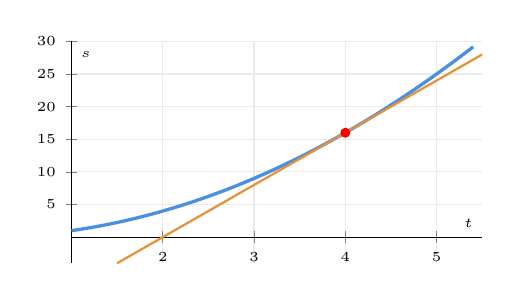
\begin{tikzpicture}\begin{axis}[width=6.8cm,height=4.4cm,axis lines=middle,xlabel={\tiny$t$},ylabel={\tiny$s$},grid=both,grid style={gray!16},xmin=1,xmax=5.5,ymin=-4,ymax=30,xtick distance=1,ytick distance=5,tick label style={font=\tiny},axis line style={-},samples=120]\addplot[exblue,very thick,domain=1:5.4]{x^2};\addplot[qorange,thick,domain=1.5:5.5]{8*x-16};\addplot[red,only marks,mark=*,mark size=1.6pt] coordinates {(4,16)};\end{axis}\end{tikzpicture}\end{center}
\end{example}

\begin{example}{ex6}{Example 7 --- Average rate (cubic)}
Average rate of change of $f(x)=x^3$ on $[1,2]$.\soln
\textbf{Step 1 (evaluate the endpoints):} $f(1)=1^3=1$ and $f(2)=2^3=8$.\\[3pt]
\textbf{Step 2 (apply the formula):} $\dfrac{f(2)-f(1)}{2-1}=\dfrac{8-1}{1}$.\\[3pt]
\textbf{Step 3 (simplify):} $=7$.\\[3pt]
\textbf{Conclusion:} average rate $=7$ --- the secant through $(1,1)$ and $(2,8)$:\eplot{0}{2.5}{-2}{10}{\addplot[exblue,very thick,domain=0:2.15]{x^3};\addplot[qorange,thick,domain=0:2.5]{7*x-6};\addplot[red,only marks,mark=*,mark size=1.6pt] coordinates {(1,1) (2,8)};}
\end{example}

\begin{example}{ex7}{Example 8 --- Velocity from a model --- estimated}
A ball's height is $h(t)=20t-5t^2$. Estimate its instantaneous velocity at $t=1$ using $h=0.001$.\soln
\textbf{Step 1 (plug into the difference quotient):} $\dfrac{h(1.001)-h(1)}{0.001}=\dfrac{[20(1.001)-5(1.001)^2]-[20(1)-5(1)^2]}{0.001}$.\\[3pt]
\textbf{Step 2 (compute each height):} $h(1.001)=20.02-5.010005=15.009995$ and $h(1)=20-5=15$.\\[3pt]
\textbf{Step 3 (subtract and divide):} $\dfrac{15.009995-15}{0.001}=\dfrac{0.009995}{0.001}=9.995$.\\[3pt]
\textbf{Conclusion:} $\approx10$ m/s --- the near-tangent line at $t=1$:\begin{center}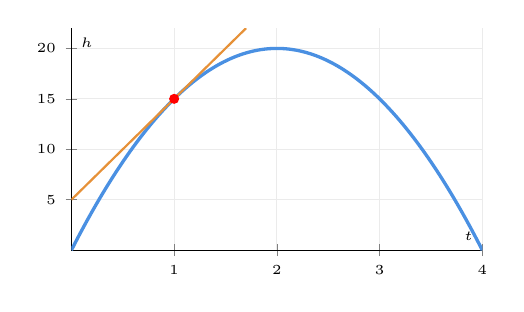
\begin{tikzpicture}\begin{axis}[width=6.8cm,height=4.4cm,axis lines=middle,xlabel={\tiny$t$},ylabel={\tiny$h$},grid=both,grid style={gray!16},xmin=0,xmax=4,ymin=0,ymax=22,xtick distance=1,ytick distance=5,tick label style={font=\tiny},axis line style={-},samples=120]\addplot[exblue,very thick,domain=0:4]{20*x-5*x^2};\addplot[qorange,thick,domain=0:1.7]{10*x+5};\addplot[red,only marks,mark=*,mark size=1.6pt] coordinates {(1,15)};\end{axis}\end{tikzpicture}\end{center}
\end{example}

\begin{example}{ex8}{Example 9 --- Difference quotient}
Simplify the difference quotient of $f(x)=2x^2$ at $x=1$.\soln
\textbf{Step 1 (form the quotient):} $\dfrac{f(1+h)-f(1)}{h}=\dfrac{2(1+h)^2-2(1)^2}{h}$.\\[3pt]
\textbf{Step 2 (expand):} $2(1+h)^2=2(1+2h+h^2)=2+4h+2h^2$, so the numerator is $2+4h+2h^2-2=4h+2h^2$.\\[3pt]
\textbf{Step 3 (factor and cancel $h$):} $\dfrac{4h+2h^2}{h}=\dfrac{h(4+2h)}{h}=4+2h$.\\[3pt]
\textbf{Conclusion:} the difference quotient simplifies to $4+2h$.
\end{example}

\clearpage
\sech{Your Turn --- Show Your Work}
For each question, show all steps clearly in the space provided.

\begin{qbox}{Question 1}
Average rate of change of $f(x)=x^2-3$ on $[2,5]$?\workspace{2.4cm}
\end{qbox}

\begin{qbox}{Question 2}
Average rate of change of $f(x)=x^2$ on $[0,4]$?\workspace{2.4cm}
\end{qbox}

\begin{qbox}{Question 3}
Simplify the difference quotient of $f(x)=x^2$ at $x=3$.\workspace{2.4cm}
\end{qbox}

\begin{qbox}{Question 4}
Estimate the instantaneous rate of $f(x)=x^2$ at $x=5$ using $h=0.001$?\workspace{2.4cm}
\end{qbox}

\begin{qbox}{Question 5}
Estimate the instantaneous rate of $f(x)=4x^2$ at $x=1$ using $h=0.001$?\workspace{2.4cm}
\end{qbox}

\begin{qbox}{Question 6}
For $s(t)=t^2$, estimate the instantaneous velocity at $t=6$ using $h=0.001$?\workspace{2.4cm}
\end{qbox}

\begin{qbox}{Question 7}
Average rate of change of $f(x)=x^3$ on $[0,2]$?\workspace{2.4cm}
\end{qbox}

\begin{qbox}{Question 8}
Simplify $\dfrac{3(2+h)^2-12}{h}$.\workspace{2.4cm}
\end{qbox}

\begin{qbox}{Question 9}
A ball's height is $h(t)=30t-5t^2$; estimate its instantaneous velocity at $t=2$ using $h=0.001$?\workspace{2.4cm}
\end{qbox}

\begin{qbox}{Question 10}
Average rate of change of $f(x)=2x+1$ on $[1,4]$?\workspace{2.4cm}
\end{qbox}

\begin{qbox}{Question 11}
Estimate the instantaneous rate of $f(x)=x^2$ at $x=-3$ using $h=0.001$?\workspace{2.4cm}
\end{qbox}

\begin{qbox}{Question 12}
For $s(t)=t^2+t$, estimate the instantaneous velocity at $t=1$ using $h=0.001$?\workspace{2.4cm}
\end{qbox}

\begin{qbox}{Question 13 --- Challenge}
A population is $P(t)=100+t^2$; estimate its instantaneous rate of growth at $t=5$ using $h=0.001$.\workspace{3cm}
\end{qbox}

\clearpage
\sech{Question Recap \& Answer Key}

\begin{recapbox}
\begin{multicols}{2}
\small
\begin{enumerate}[leftmargin=*,itemsep=3pt]
  \item Average rate of change of $f(x)=x^2-3$ on $[2,5]$?
  \item Average rate of change of $f(x)=x^2$ on $[0,4]$?
  \item Simplify the difference quotient of $f(x)=x^2$ at $x=3$.
  \item Estimate the instantaneous rate of $f(x)=x^2$ at $x=5$ using $h=0.001$?
  \item Estimate the instantaneous rate of $f(x)=4x^2$ at $x=1$ using $h=0.001$?
  \item For $s(t)=t^2$, estimate the instantaneous velocity at $t=6$ using $h=0.001$?
  \item Average rate of change of $f(x)=x^3$ on $[0,2]$?
  \item Simplify $\dfrac{3(2+h)^2-12}{h}$.
  \item A ball's height is $h(t)=30t-5t^2$; estimate its instantaneous velocity at $t=2$ using $h=0.001$?
  \item Average rate of change of $f(x)=2x+1$ on $[1,4]$?
  \item Estimate the instantaneous rate of $f(x)=x^2$ at $x=-3$ using $h=0.001$?
  \item For $s(t)=t^2+t$, estimate the instantaneous velocity at $t=1$ using $h=0.001$?
  \item A population is $P(t)=100+t^2$; estimate its instantaneous rate of growth at $t=5$ using $h=0.001$.
\end{enumerate}
\end{multicols}
\end{recapbox}

\begin{keybox}
\begin{multicols}{2}
\small
\begin{enumerate}[leftmargin=*,itemsep=3pt]
  \item $\tfrac{22-1}{3}=7$
  \item $4$
  \item $6+h$
  \item $\approx10$
  \item $\approx8$
  \item $\approx12$
  \item $\tfrac{8-0}{2}=4$
  \item $12+3h$
  \item $\approx10$ m/s
  \item $2$
  \item $\approx-6$
  \item $\approx3$
  \item $\approx10$
\end{enumerate}
\end{multicols}
\end{keybox}

\end{document}
